\scanpage{21}
% archive sheet number: 20

\figure{\begin{tikzpicture}[x=.00555cm,y=-.00555cm,line cap=round,line join=round,inner sep=.4pt]
% Drawing 1
\begin{scope}
\draw (54,274)--(329,81) (57,244)--(380,117) (149,82)--(344,285) (233,34)..controls(269,133)and(300,228)..(331,358);
\draw (527,62)--(525,515) (538,62)..controls(551,156)and(534,382)..(541,530);
\node[scale=0.8,transform shape=false] at (176,357) {$4$};
\node[scale=0.7,transform shape=false] at (327,418) {$(\mathfrak S_{\unsure{4|1}})$};
\node[scale=0.75,transform shape=false] at (196,519) {$(1)$};
\end{scope}
% Drawing 2
\begin{scope}
\draw (628,297)--(982,131) (694,284)--(921,87) (692,135)..controls(807,134)and(954,168)..(1064,171) (762,105)..controls(791,86)and(863,211)..(992,334) (844,56)..controls(870,151)and(972,336)..(1005,442);
\node[scale=0.72,transform shape=false] at (828,361) {$5\ \mathrm{pos.}$};
\node[scale=0.68,transform shape=false] at (775,427) {$(D_5)\quad\text{générale}$};
\node[scale=0.52,transform shape=false] at (1093,477) {$\deleted{\unsure{\mathfrak S_5^{*}}}$};
\node[scale=0.72,transform shape=false] at (848,555) {$(2)$};
\end{scope}
% Drawing 3
\begin{scope}
\draw (1200,285)--(1555,110) (1226,291)--(1482,53) (1331,331)..controls(1377,247)and(1429,113)..(1472,27) (1372,49)--(1497,325) (1424,29)--(1513,407);
\node[scale=0.7,transform shape=false] at (1382,399) {$5\ \text{position}$};
\node[scale=0.7,transform shape=false] at (1385,475) {$\text{particulière}$};
\node[scale=0.72,transform shape=false] at (1358,574) {$(3)$};
\end{scope}
% Drawing 4
\begin{scope}
\draw (1729,316)..controls(1852,313)and(1990,297)..(2139,290) (1732,353)--(2096,159) (1760,361)--(1973,112) (1816,183)--(2145,343) (1922,93)--(2101,390) (1935,355)..controls(1946,283)and(1944,153)..(1956,87);
\foreach \x/\y in {1807/311,1945/236,1953/134,2052/295}{\fill (\x,\y) circle (7);}
\node[scale=0.7,transform shape=false] at (2016,406) {$6\ \text{en position}$};
\node[scale=0.69,transform shape=false] at (2030,457) {$\text{\unsure{tétraédrale|tétraèdrale}}$};
\node[scale=0.72,transform shape=false] at (1930,519) {$(4)$};
\end{scope}

\end{tikzpicture}}

Tout arrangement 1-dim. de ps. droites \deleted{qui \unsure{est un}} \deleted{\unsure{contient}} \unsure{provenant|pouvant|comportant} \deleted{\unsure{plan|des|être}} de ps. droites bigonal, \deleted{contient une des $4$ configurations} \inserted{si elle n'est réduit à $4$ ps droites (auquel cas c'est le cas (1))} contient une des \inserted{types de} configurations (2) (3) (4) qui sont \deleted{``spéciales'', \unsure{soit}} ``non spéciales'', i.e. quand elles sont réalisées par des arrangements \inserted{2-dim.} de ps. droites, alors l'intersection de deux faces fermées est \deleted{une face,} vide, réduite à un sommet, ou est une arête fermée.

\uline{NB} Si elle ne contient (2) ni (3), alors \deleted{c'est} elle est du type (4), ou du type (5)

\figure{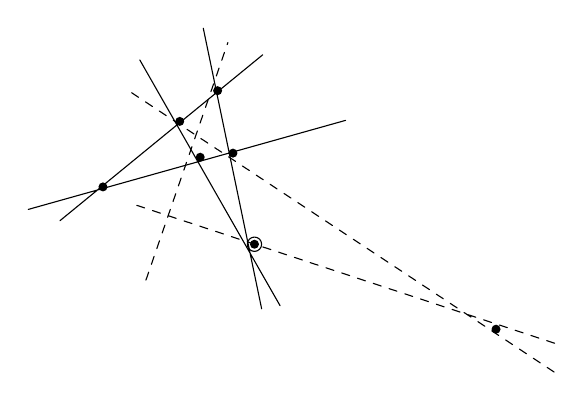
\begin{tikzpicture}[x=0.013cm,y=-0.013cm,line cap=round,line join=round,inner sep=0.4pt]
\draw (1111,1433)--(1421,1346) (1142,1444)--(1340,1282) (1220,1287)--(1357,1527) (1282,1256)--(1339,1530);
\draw[dashed] (1212,1319)--(1628,1594) (1226,1502)--(1306,1270) (1217,1429)--(1626,1564);
\foreach \x/\y in {1184/1411,1259/1347,1296/1317,1279/1382,1311/1378,1332/1467,1568/1550}{\fill (\x,\y) circle (4.4);}
\draw (1332,1467) circle (7);

\end{tikzpicture}}

de $7$ ps. droites formé d'un quadrilatère et de trois diagonales, qui mérite d'être étudié

\deleted{Si elle ne contient}
